% BLG558E Term Project - Assignment 2 skeleton (IEEE conference format).
% Content is intentionally EMPTY: the assignment requires you to write the text yourself, in your own words.
% If Ninova provides its own template, copy the section structure below into that template.
%
% Requirements from the assignment PDF (check before submitting):
%  - IEEE Conference Paper format, PDF, 5 to 5.5 pages (at least 5 FULL pages)
%  - Title, authors, address, e-mail
%  - Abstract: max 150 words
%  - Introduction (~1 page including title and abstract): the subject, its importance, what has been done in your paper
%  - Related Work: give it a SPECIFIC name (max 1 page)
%  - Proposed solution: give it a SPECIFIC name (at least 1 page)
%  - Analysis of your proposed solution (at least 1 page)
%  - Conclusion and Future Work: problem, solution, contributions (less than half a page)
%  - References: 10 to 15, at least 5 journal papers published since 2024;
%    open sources (web pages, newsletters, technical reports) are NOT accepted
%  - Not a survey paper. Do not copy-paste; do not use AI tools for summary or content.
\documentclass[conference]{IEEEtran}
\IEEEoverridecommandlockouts
\usepackage{cite}
\usepackage{amsmath,amssymb,amsfonts}
\usepackage{graphicx}
\usepackage{booktabs}
\usepackage{xcolor}

\begin{document}

\title{[Paper Title]}

\author{\IEEEauthorblockN{[Name Surname]}
\IEEEauthorblockA{[Department, Istanbul Technical University]\\
[City, Country]\\
[email@itu.edu.tr]}}

\maketitle

\begin{abstract}
% max 150 words
[Write your abstract here.]
\end{abstract}

\begin{IEEEkeywords}
[keyword 1, keyword 2, keyword 3, keyword 4]
\end{IEEEkeywords}

\section{Introduction}
% ~1 page including title and abstract.
% Answer: what is the subject? why is it important? what has been done in this paper?
[Write here.]

\section{[Specific Name for the Related Work Section]}
% max 1 page.
[Write here.]

\section{[Specific Name for Your Proposed Solution]}
% at least 1 page.
[Write here.]

% Optional drop-in for existing result figures (uncomment and adjust the path):
% \begin{figure}[t]
%   \centering
%   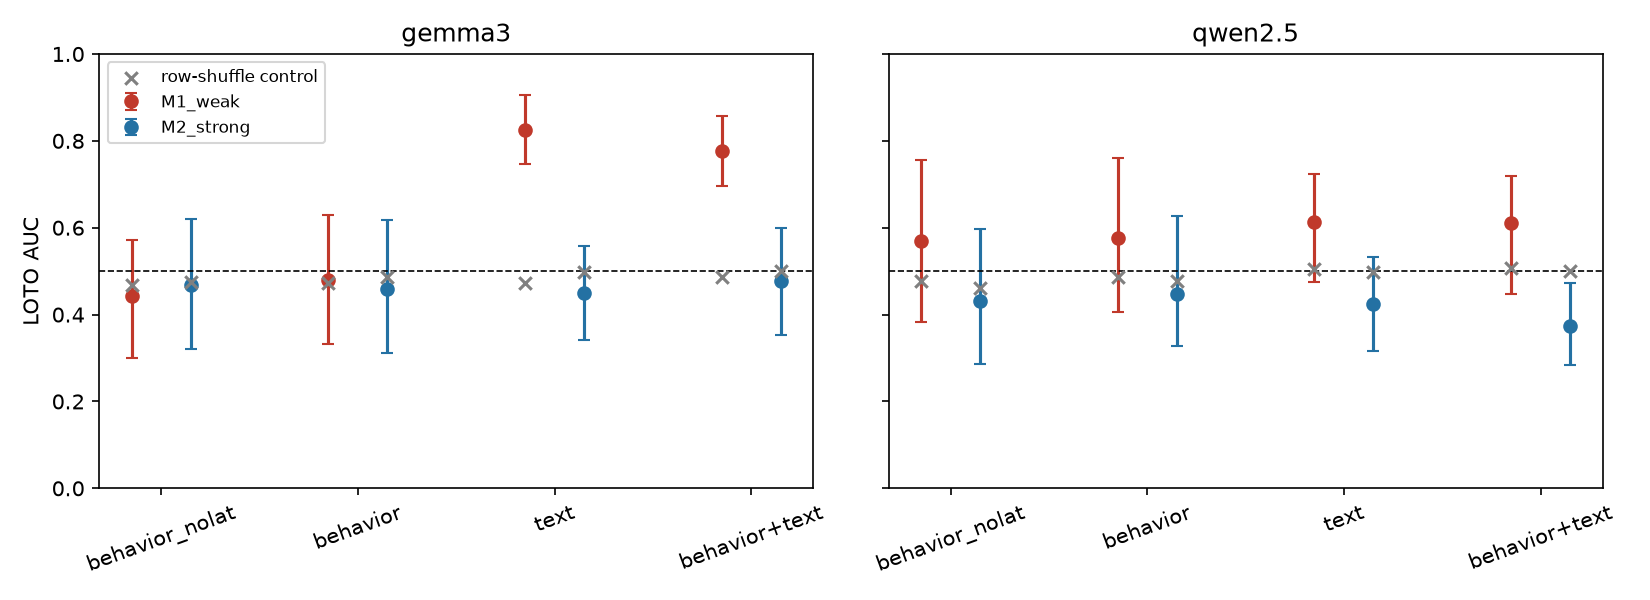
\includegraphics[width=\columnwidth]{../../results/figures/auc_m1_vs_m2.png}
%   \caption{[Caption]}
%   \label{fig:auc}
% \end{figure}

\section{Analysis of the Proposed Solution}
% at least 1 page.
[Write here.]

\section{Conclusion and Future Work}
% less than half a page: problem, solution, contributions.
[Write here.]

\begin{thebibliography}{00}
% 10 to 15 references. At least 5 journal papers published since 2024.
% See kaynak_adaylari.md for candidate sources to READ; fill each entry from the publisher page.
\bibitem{b1} [Author(s), ``Title,'' \emph{Journal/Conference}, vol., no., pp., year.]
\bibitem{b2} [ ]
\bibitem{b3} [ ]
\bibitem{b4} [ ]
\bibitem{b5} [ ]
\bibitem{b6} [ ]
\bibitem{b7} [ ]
\bibitem{b8} [ ]
\bibitem{b9} [ ]
\bibitem{b10} [ ]
\end{thebibliography}

\end{document}
